\documentclass{beamer}

\usepackage[utf8]{inputenc}
\usecolortheme{beaver}
\usepackage{caption}
\usepackage{subcaption}
\usepackage{mathtools}
\usepackage{todonotes}
\usepackage{amsmath}
\usepackage{bm}
\usepackage{listings}
\usepackage{ragged2e}
\usepackage{titlecaps}
\usepackage{fancyvrb}

\def\ci{\perp\!\!\!\!\!\perp}

\newtheorem{proposition}{Proposition}
\Addlcwords{for a is but and with of in as the etc on to if}

\setbeamertemplate{section in toc}{\inserttocsectionnumber.~\inserttocsection}
\usetheme{Boadilla}
\makeatletter
\setbeamertemplate{footline}{%
    \leavevmode%
    \hbox{%
        \begin{beamercolorbox}[wd=.3\paperwidth,ht=2.25ex,dp=1ex,center]{author in head/foot}%
            \usebeamerfont{author in head/foot}\insertshortauthor\expandafter\beamer@ifempty\expandafter{\beamer@shortinstitute}{}{~~(\insertshortinstitute)}
        \end{beamercolorbox}%
        \begin{beamercolorbox}[wd=.55\paperwidth,ht=2.25ex,dp=1ex,center]{title in head/foot}%
            \usebeamerfont{title in head/foot}\insertshorttitle
        \end{beamercolorbox}%
        \begin{beamercolorbox}[wd=.15\paperwidth,ht=2.25ex,dp=1ex,right]{date in head/foot}%
            \usebeamerfont{date in head/foot}\insertshortdate{}\hspace*{2em}
            \insertframenumber{} / \inserttotalframenumber\hspace*{2ex} 
        \end{beamercolorbox}}%
        \vskip0pt%
    }
\makeatother

\begin{document}

\title[]{Expert-in-the-Loop Causal Discovery}
\author{Ankur Ankan}
\date{}

\maketitle

\begin{frame}{Directed Acyclic Graphs (DAGs)}
	\begin{columns}
		\begin{column}{0.6 \textwidth}
		\begin{itemize}
			\item Nodes represent random variables.
			\item Edges represent causal relationships.
			\item E.g., \textbf{Education} has a direct effect on \textbf{Income}. 
			\item \textbf{Age} has indirect effect on \textbf{Income} through \textbf{Education} and \textbf{Hours Per Week}.
			\item Used for causal effect estimation.
		\end{itemize}
		\end{column}

		\begin{column}{0.45 \textwidth}
		\begin{figure}
			\centering
			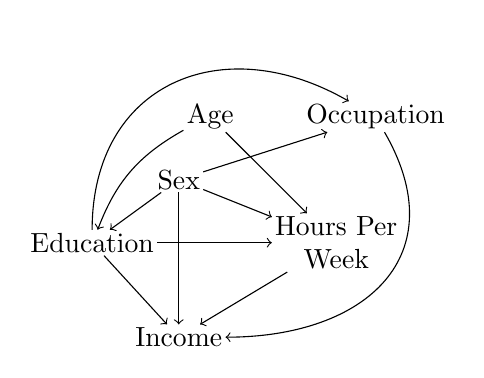
\begin{tikzpicture}[scale=1]
			\tikzstyle{every node}=[align=center, inner sep=1pt]
				\node (sex) at (-0.7, -0.8) {Sex};
				\node (age) at (-0.3, 0) {Age};
				\node (ed) at (-1.8, -1.6) {Education};
				\node (occ) at (1.8, 0) {Occupation};
				\node (hrpw) at (1.3, -1.6) {Hours Per \\ Week};
				\node (income) at (-0.7, -2.8) {Income};
			
				\draw[->]  (age) to[bend right=20] (ed);
				\draw[->]  (sex) to (ed);
				\draw[->]  (age) to (hrpw);
				\draw[->]  (ed) to (hrpw);
				\draw[->]  (sex) to (hrpw);
				\draw[->]  (ed) to (income);
				\draw[->]  (hrpw) to (income);
				\draw[->]  (occ) to[out=300, in=0, looseness=1.4] (income.east);
				\draw[->]  (sex) to (income);
				\draw[->]  (ed) to[out=90, in=150, looseness=1.3] (occ);
				\draw[->]  (sex) to (occ);	
			\end{tikzpicture}
			\caption{Example of a DAG}
		\end{figure}
		\end{column}
	\end{columns}	
\end{frame}

\begin{frame}{Causal Discovery: Learning DAGs From Observational Data}
	\begin{figure}
		\centering
		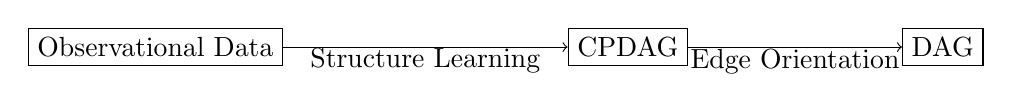
\begin{tikzpicture}
			\node[draw, rectangle] (x) at ( 0, 0 ) { Observational Data };
			\node[draw, rectangle] (y) at ( 6, 0 ) { CPDAG };
			\node[draw, rectangle] (z) at ( 10, 0) { DAG };
		
			\draw[->](x) -- (y) node[midway, below, yshift=0.1cm]{ Structure Learning };
			\draw[->](y) -- (z) node[midway, below, yshift=0.1cm]{ Edge Orientation };
		\end{tikzpicture}
	\end{figure}
	\todo[inline]{Improve the figure. Show an example right below the steps }

	\begin{itemize}
		\item Goal of Causal Discovery is to recover the DAG from data.
		\item Many algorithms are available:
			\begin{itemize}
				\item Constraint Based (PC, FCI)
				\item Score Based (Hill-Climb Search, GES)
				\item Optimization Based (No Tears)
			\end{itemize}
		\item Algorithms can only recover Markov Equivalence Class.
		\item To orient edges of CPDAG, either use expert knowledge or make some assumptions.
	\end{itemize}
\end{frame}

\begin{frame}{Causal Discovery in Practice}
	\begin{itemize}
		\item Adaption of causal discovery algorithms is very limited.
		\item Researchers prefer to draw models by hand based on domain knowledge.
		\item Potential reasons could be:
			\begin{itemize}
				\item Algorithms can make obvious mistakes, making it harder to trust.
				\item Hard to choose an algorithm for a given dataset because of the different assumptions.
				\item No way to evaluate algorithm performance on a given dataset.
			\end{itemize}
		\item However, some researchers do test their model against data.
	\end{itemize}
\end{frame}

\begin{frame}{Model Testing Using Conditional Independence (CI) Tests}
	\todo[inline]{Add an example of model testing here}

	\begin{itemize}
		\item Each missing edge in the model imply a conditional independence (CI) statement. \todo[inline]{Double check this statement}
		\item We can test these in the given data to verify if the model agrees with the data.
		\item If the test fails, it implies that the correlation between the variables is not explained by the model.
		\item These tests can be used to iteratively modify the network.
	\end{itemize}
\end{frame}

\begin{frame}{Deciding edges between variables based on effect sizes}
	The CI tests gives an effect size that can be used to decide whether an edge exists or not.

	\todo[inline]{Show an example of the mediator model here to explain how can we decide}
\end{frame}

\begin{frame}{Human-in-the-loop Structure Learning}
	A browser based tool to assist with drawing DAGs.
	\begin{itemize}
		
	\end{itemize}
\end{frame}

\begin{frame}{Show an example of how this works}
\end{frame}

\begin{frame}{Effect Size For Continuous Variables}
	For continuous variable partial correlations is typically used.

	For discrete variables Cramer's V can be used.

	We propose an effect size based on canonical correlations that can work on any mixture of variables.
\end{frame}

\begin{frame}{Effect Size: Marginal Case}
	We have two cases, first marginal when we have no conditional variables.

	Canonical Correlations have some nice properties: 1) Reduces down to know effect size measures in standard cases. 2) Bounded between $ 0 $ and $ 1 $.

	For discrete variables, we dummy encode them and take the canonical correlation based effect size.

	For continuous variable, we take the canoncial correlations simply.
\end{frame}

\begin{frame}{Effect Size: Conditional Case}
	If the continuous case partial correlation is used typically. Partial correlaton is computed using two regression methods and taking the correlation between the residuals.

	We extend this to mixed data case as well by using regression to comput the residuals, and then taking the canonical correlation based effect size.
\end{frame}

\begin{frame}{Empirical Analysis}
	To compare how well this approach works compared to the algorithms.

	But need to simulate an expert/human:
	\begin{itemize}
		\item Take a greedy approach and choose the variables with the highest effect between them such that it does not create a cycle.
		\item Use an oracle with a given accuracy to determine the direction of the edge.
		\item After each edge addition the effects are recomputed.
		\item A pruning step is done to check if adding an edge removes some of the effects.
	\end{itemize}
\end{frame}

\begin{frame}{Empirical Analysis}
	\begin{itemize}
		\item Generate random DAGs on $10$ nodes.
		\item Linear Mixed data is simulated from these DAGs.
		\item We use the PC, Hill-Climb, and expert simulator to learn the original DAG.
		\item Compare the Structural Hamming Distance (SHD) and Structural Intervention Distance (SID) between the true and the learned graph.
		\item Because PC and Hill-Climb can only learn CPDAGs, we show the results using best and worst performing DAG orientations.
	\end{itemize}
\end{frame}


\begin{frame}{Empirical Analysis: Structural Hamming Distance}
	\begin{figure}
		\centering
		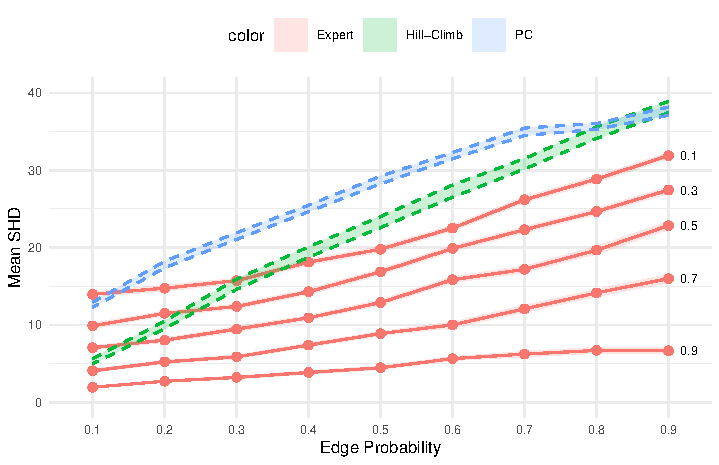
\includegraphics[scale=0.9]{../../2024-human-sl/code/plots/shd_ribbon.pdf}
		\caption{SHD vs edge probability}
	\end{figure}
\end{frame}

\begin{frame}{Empirical Analysis: Structural Hamming Distance}
	\begin{figure}
		\centering
		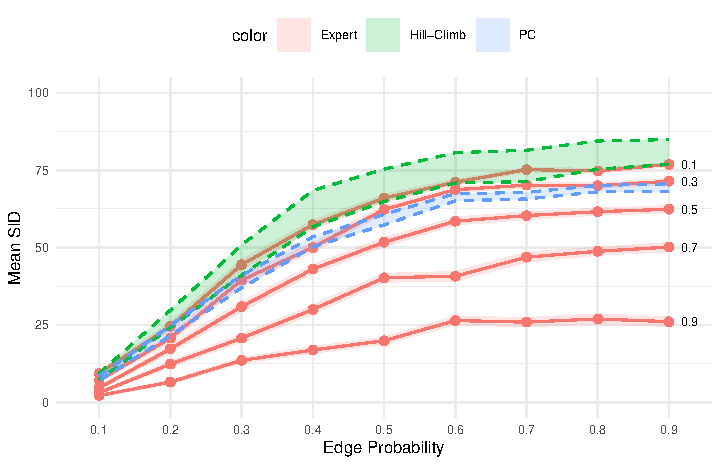
\includegraphics[scale=0.9]{../../2024-human-sl/code/plots/sid_ribbon.pdf}
		\caption{SID vs edge probability}
	\end{figure}
\end{frame}

\begin{frame}{LLMs as Oracles}
\end{frame}

\begin{frame}{Conclusion}
	\begin{itemize}
		\item We built a tool to interactively draw DAGs combining it with model testing.
		\item We propose an effect size measure for mixed data.
		\item For oracles with reasonable accuracy we are able more accurate DAGs.
		\item The human simulator can get stuck in local minimas. Actual humans should perform better.
		\item Oracles can be replaced with LLMs.
	\end{itemize}
\end{frame}

\end{document}
